\documentclass{beamer}

\mode<presentation>
{
  \usetheme{Warsaw}
  % or ...

  \setbeamercovered{transparent}
  % or whatever (possibly just delete it)
}


\usepackage[english]{babel}
\usepackage[latin1]{inputenc}
\usepackage{graphicx}
%\usepackage{times}
%\usepackage[T1]{fontenc}
% Or whatever. Note that the encoding and the font should match. If T1
% does not look nice, try deleting the line with the fontenc.

\usepackage{amsmath,amsfonts,amssymb}

\newcommand{\pkg}{\textbf}
\newcommand{\code}{\texttt}
\newcommand{\bsym}{\boldsymbol}
\newcommand{\eps}{\varepsilon}
\newcommand{\bx}{\mathbf{x}}
\newcommand{\bX}{\mathbf{X}}
\newcommand{\bZ}{\mathbf{Z}}
\newcommand{\bz}{\mathbf{z}}
\newcommand{\newp}{\vspace{1em}}
\newcommand{\Var}{\text{Var}}
\newcommand{\PMTen}{PM$_{10}$}
\newcommand{\Cov}{\text{Cov}}
\newcommand{\bi}{\begin{itemize}}
\newcommand{\ei}{\end{itemize}}


\title{Regular Expressions}

\subtitle{(special thanks to Mark Hansen)}

\date{Biostatistics 140.776}

\begin{document}

\begin{frame}
  \titlepage
\end{frame}

\begin{frame}{Listening Post}
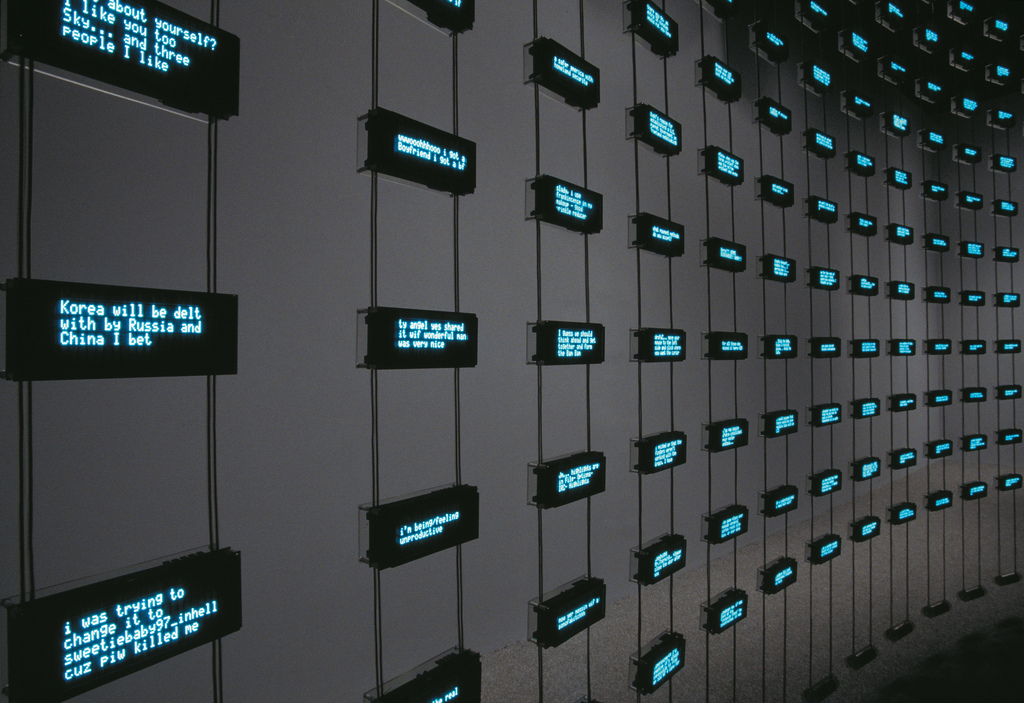
\includegraphics[height=3in]{listeningpost}
\end{frame}

\begin{frame}{Moveable Type}
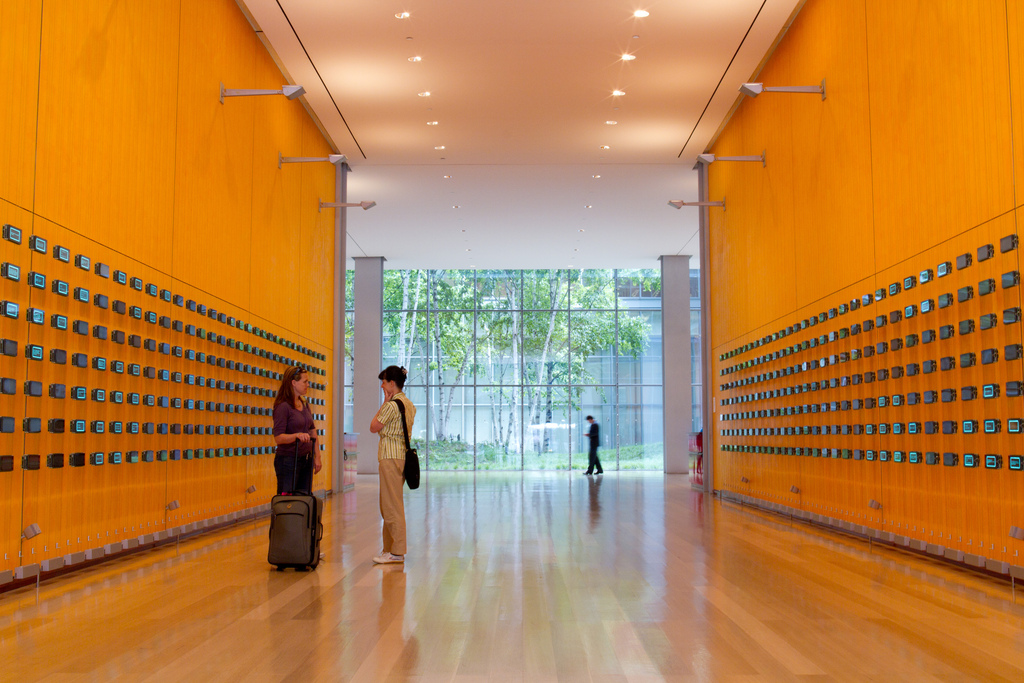
\includegraphics[height=3in]{MT1}
\end{frame}

\begin{frame}{Moveable Type}
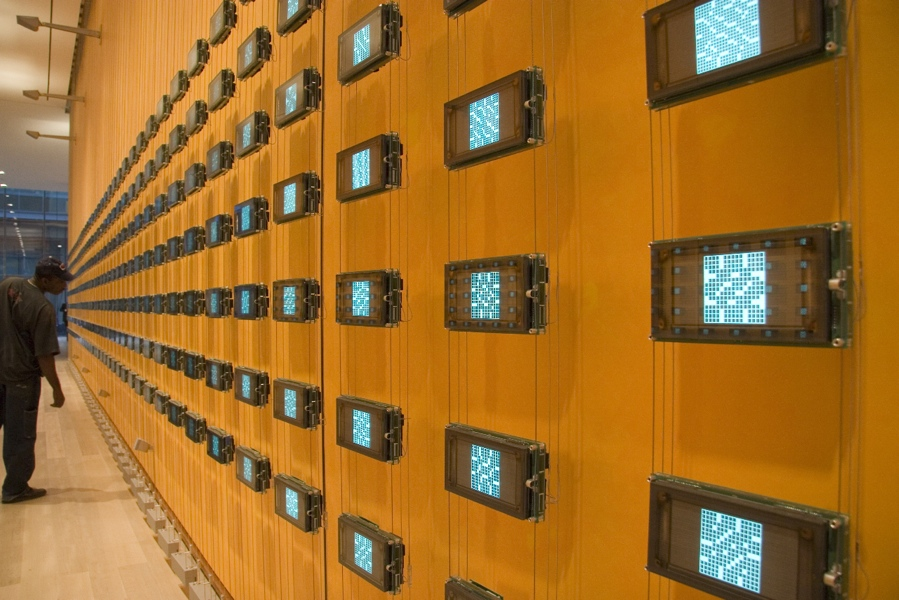
\includegraphics[height=3in]{MT2}
\end{frame}

\begin{frame}{Regular expressions}
\begin{itemize}
\item
Regular expressions can be thought of as a combination of literals and
\textit{metacharacters}
\item
To draw an analogy with natural language, think of literal text
forming the words of this language, and the metacharacters defining
its grammar
\item
Regular expressions have a rich set of metacharacters
\end{itemize}

\end{frame}

\begin{frame}[fragile]{Literals}
Simplest pattern consists only of literals.  The literal ``nuclear''
would match to the following lines:
\begin{verbatim}
Why do we trust our government with 8,500 nuclear weapons, 
but not to administer health care?

Beginning to regret that nuclear taco

Apple is all about nuclear family level network effects.

"I'm going to destroy Android, because it's a stolen 
product. I'm willing to go thermonuclear war on 
this." - Steve Jobs
\end{verbatim}
\end{frame}

\begin{frame}[fragile]{Literals}
The literal ``Obama'' would match to the following lines
\begin{verbatim}
I am going to take so many pictures of Michelle Obama 
today...

It's Official...The USA Has Been Renamed. It is Now 
the USSR (United States Socialist Republic) 
Thanks Mr Obama.

I'm #Obama all the way I think 4 years is too short 
to be in office

Obama's budget was rejected by the Senate 99 - 0.
\end{verbatim}
\end{frame}

\begin{frame}{Regular Expressions}
\begin{itemize}
\item
Simplest pattern consists only of literals; a match occurs if the
sequence of literals occurs anywhere in the text being tested
\item
What if we only want the word ``Obama'', but no hashtags? Or sentences that end in 
the word ``Clinton'', or ``clinton''? 
\end{itemize}
\end{frame}

\begin{frame}{Regular Expressions}
We need a way to express
\begin{itemize}
\item
whitespace word boundaries
\item
sets of literals
\item
the beginning and end of a line
\item
alternatives (``war'' or ``peace'')
\end{itemize}
Metacharacters to the rescue!
\end{frame}

\begin{frame}[fragile]{Metacharacters}
Some metacharacters represent the start of a line
\begin{verbatim}
^i think 
\end{verbatim}
will match the lines 
\begin{verbatim}
i think should text me.

i think i lost my laptop...

i think "hipster shorts" are the ugliest stupidest 
things ever

i think i'm gonna go for a run after work 
today.....i think....=\
\end{verbatim}
\end{frame}

\begin{frame}[fragile]{Metacharacters}
\$ represents the end of a line
\begin{verbatim}
morning$ 
\end{verbatim}
will match the lines 
\begin{verbatim}
i hate parting ways with my blankie in the morning

#oomf is cracking me up this morning

so watsup this morning

No plans tonight have to be to work to early in the morning

Nothin like sprinting after a bus on a Tuesday morning
\end{verbatim}
\end{frame}

\begin{frame}[fragile]{Character Classes with []}
We can list a set of characters we will accept at a given point in the
match
\begin{verbatim}
[Bb][Uu][Ss][Hh]
\end{verbatim}
will match the lines 
\begin{verbatim}
Headed to King George to be with Pern, & Bushel of 
whole crabs waiting and doing some party planning!

Eco design pioneer Barbara Dornbush speaking 
June 17 11:30AM at Verde Home in Westside.

Kanye's as stupid as Bush.

is bush league ..... thanks for nothing!
\end{verbatim}
\end{frame}

\begin{frame}[fragile]{Character Classes with []}
\begin{verbatim}
^[Ii] am
\end{verbatim}
will match
\begin{verbatim}
I am BEYOND irritated right now

i am boycotting the apple store

I am twittering from iPhone

i am going to dream in XML tonight. ugh.

I am so over this. I need food. Mmmm bacon...
\end{verbatim}
\end{frame}

\begin{frame}[fragile]{Character Classes with []}
Similarly, you can specify a range of letters [a-z] or 
[a-zA-Z]; notice that the order doesn't matter
\begin{verbatim}
^[0-9][a-zA-Z]
\end{verbatim}
will match the lines 
\begin{verbatim}
7th inning stretch
2nd half soon to begin. OSU did just win something
3am - cant sleep - too hot still.. :(
5ft 7 sent from heaven 
1st sign of starvagtion
\end{verbatim}
\end{frame}

\begin{frame}[fragile]{Character Classes with []}
When used at the beginning of a character class, the ``\verb+^+'' is also a 
metacharacter and indicates matching characters NOT in the 
indicated class
\begin{verbatim}
[^?.]$
\end{verbatim}
will match the lines 
\begin{verbatim}
i like basketballs 
6 and 9
dont worry... we all die anyway! 
Not in Baghdad
helicopter under water? hmmm
\end{verbatim}
\end{frame}

\begin{frame}[fragile]{More Metacharacters}
``.'' is used to refer to any character. So
\begin{verbatim}
9.11
\end{verbatim}
will match the lines 
\begin{verbatim}
With the anniversary of 9/11 coming up, I just 
wanted to wish the world some Peace.

tune in tomorrow morning(9-11)to The Weekend Sports 
Buzz on 1450am

why do i ALWAYS look at the clock at 1:43 and 9:11?????

Stock up now for the holidays at Siesel's Meats 
in San Diego, CA 92110
\end{verbatim}
\end{frame}

\begin{frame}[fragile]{More Metacharacters: $|$}
The $|$ character indicates a logical ``or''; we can use it to combine two
expressions, the subexpressions being called alternatives
\begin{verbatim}
flood|fire
\end{verbatim}
will match the lines 
\begin{verbatim}
eating some firehouse subs. m m

On way home drove by flooding areas of the San Diego 
River, was okay then, but how long will it be okay 
with the rain still coming down?

Between you and me, there are wildfires.
\end{verbatim}
\end{frame}

\begin{frame}[fragile]{More Metacharacters: $|$}
We can include any number of alternatives...
\begin{verbatim}
flood|earthquake|hurricane|coldfire
\end{verbatim}
will match the lines 
\begin{verbatim}
Not a whole lot of hurricanes in the Arctic.

We do have earthquakes nearly every day somewhere 
in our State 

hurricanes swirl in the other direction 

coldfire is STRAIGHT! 

'cause we keep getting earthquakes
\end{verbatim}
\end{frame}

\begin{frame}[fragile]{More Metacharacters: $|$}
The alternatives can be real expressions and not just literals
\begin{verbatim}
^[Gg]ood|[Bb]ad
\end{verbatim}
will match the lines 
\begin{verbatim}
Good morning tweeps

goodnight handsome <3

this is a bad idea for Netflix

Not a bad way to put it. Content has to be useful 
to work, and must serve our readers and users.
\end{verbatim}
\end{frame}

\begin{frame}[fragile]{More Metacharacters: ( and )}
Subexpressions are often contained in parentheses to constrain the 
alternatives
\begin{verbatim}
^([Gg]ood|[Bb]ad)
\end{verbatim}
will match the lines 
\begin{verbatim}
good for you!

Good. How is the house

Bad dreams are overrated.

Badger Herald uses really weak reasoning in Op-Ed
\end{verbatim}
\end{frame}

\begin{frame}[fragile]{More Metacharacters: ?}
The question mark indicates that the indicated expression is optional
\begin{verbatim}
[Gg]eorge( [Ww]\.)? [Bb]ush
\end{verbatim}
will match the lines 
\begin{verbatim}
i bet i can spell better than you and george bush combined

BBC reported that President George W. Bush claimed 
God told him to invade Iraq 

a bird in the hand is worth two george bushes 
\end{verbatim}
\end{frame}

\begin{frame}[fragile]{One thing to note...}
In the following
\begin{verbatim}
[Gg]eorge( [Ww]\.)? [Bb]ush
\end{verbatim}
we wanted to match a ``.'' as a literal period; to do that, we had to
``escape'' the metacharacter, preceding it with a backslash In
general, we have to do this for any metacharacter we want to include
in our match
\end{frame}

\begin{frame}[fragile]{More metacharacters: * and +}
The * and + signs are metacharacters used to indicate repetition; * 
means ``any number, including none, of the item'' and + means ``at 
least one of the item''
\begin{verbatim}
\(.*\)
\end{verbatim}
will match the lines 
\begin{verbatim}
anyone wanna chat? (24, m, germany)

hello, 20.m here... ( east area + drives + webcam ) 

(he means older men) 

()
\end{verbatim}
\end{frame}

\begin{frame}[fragile]{More metacharacters: * and +}
The * and + signs are metacharacters used to indicate repetition; * 
means ``any number, including none, of the item'' and + means ``at 
least one of the item''
\begin{verbatim}
[0-9]+ (.*)[0-9]+
\end{verbatim}
will match the lines 
\begin{verbatim}
working as MP here 720 MP battallion, 42nd birgade 

so say 2 or 3 years at colleage and 4 at uni makes us 23 
when and if we finish

it went down on several occasions for like, 3 or 4 *days*

Mmmm its time 4 me 2 go 2 bed
\end{verbatim}
\end{frame}

\begin{frame}[fragile]{More metacharacters: \{ and \}}
\{ and \} are referred to as interval quantifiers; the let us specify
the minimum and maximum number of matches of an expression
\begin{verbatim}
[Oo]bama( +[^ ]+){1,5} debate
\end{verbatim}
will match the lines 
\begin{verbatim}
why is it every time I hear Newt speak I want to vote for 
him? He would crush Obama in a debate

One Gaddafi moment for Obama was worth all the debates 
put together!

Romney + Obama should debate using the universal language 
of music via that contraption Dick Van Dyke wore in Mary 
Poppins

#Obama and #Boehner could settle #debtlimit debate once 
and for all w/ an old fashioned staring contest.
\end{verbatim}
\end{frame}

\begin{frame}[fragile]{More metacharacters: \{ and \}}
\begin{itemize}
\item
\{m,n\} means at least m but not more than n matches
\item
\{m\} means exactly m matches
\item
\{m,\} means at least m matches
\item \{,n\} means at most n matches
\end{itemize}
\end{frame}

\begin{frame}[fragile]{More metacharacters: ( and ) revisited}
\begin{itemize}
\item
In most implementations of regular expressions, the parentheses not
only limit the scope of alternatives divided by a ``$|$'', but also
can be used to ``remember'' text matched by the subexpression enclosed
\item
We refer to the matched text with \verb+\1+, \verb+\2+, etc.
\end{itemize}
\end{frame}

\begin{frame}[fragile]{More metacharacters: ( and ) revisited}
So the expression 
\begin{verbatim}
 +([a-zA-Z]+) +\1 +
\end{verbatim}
will match the lines 
\begin{verbatim}
time for bed, night night twitter!

blah blah blah blah 

my tattoo is so so itchy today

i was standing all all alone against the world outside...

hi anybody anybody at home

estudiando css css css css.... que desastritooooo
\end{verbatim}
\end{frame}

\begin{frame}[fragile]{More metacharacters: ( and ) revisited}
The \verb+*+ is ``greedy'' so it always matches the \textit{longest}
possible string that satisfies the regular expression. So
\begin{verbatim}
^s(.*)s
\end{verbatim}
matches
\begin{verbatim}
sitting at starbucks

setting up mysql and rails

studying stuff for the exams

spaghetti with marshmallows

stop fighting with crackers

sore shoulders, stupid ergonomics
\end{verbatim}
\end{frame}

\begin{frame}[fragile]{More metacharacters: ( and ) revisited}
The greediness of \verb+*+ can be turned off with the \verb+?+, as in
\begin{verbatim}
^s(.*?)s
\end{verbatim}
\end{frame}

\begin{frame}{Summary}
Regular expressions consist of
\begin{itemize}
\item Literals, strings of characters
\item Character classes
\item General metacharacters, descriptions of complex word/symbol combinations 
\end{itemize}
\end{frame}



\end{document}
